%!TEX root = ../main.tex

\chapter{为何使用\LaTeX 排版学位论文\footnote{请不要在正式论文撰写中如本文般滥用脚注}}
% 原则上,每一章开头不可马上进入第一节
% 需要一段引文提要起到 TL;DR 的作用
不同往日,在国内使用 Unix 类操作系统尤其是 OS X 的同学越来越多,
而学校发布文档模板时仍旧大多使用微软办公套件。
在这种矛盾下,
惯用Unix系的同学在通过兼容方案打开或编辑文档时遭遇诸多不便,
甚至被迫切换到虚拟机环境下撰写论文。
鉴于此,本模板解决的首要问题即是:
\textbf{使用OS X的同学如何完全脱离windows环境完成论文撰写工作}。

对于未参与长期科研工作且惯用 windows 操作系统的国内大学生而言,
提到“排版”,仅能考虑到的工具几乎只有微软公司的字处理软件Word系列。
然而,讽刺的是,熟练掌握 Word 系列工具的同学并不占多数。
在下曾参与软件学院论文格式审查工作,
发现相当一部分同学对排版知识了解甚少,
字体、目录、图片、参考文献皆混乱不堪。
分析其中原因,窃以为有以下几条:
\begin{enumerate}
    \item 对论文撰写工作不够重视,将学位论文当成项目报告
    \item office系列软件的“易用性”导致了在工具使用上的心理轻视
    \item 缺乏排版常识
\end{enumerate}

工具本身并无高低贵贱之分,
无论您使用何种工具,都有方法高效地排版一份精美的论文。
使用\LaTeX \footnote{知道准确的\LaTeX 发音的不必嘲笑将它念成leiteks的人}
并不是以此体现自己高人一等的装x行为\footnote{此处不讨论鄙视链和党争等哲学话题},
参看王垠的《谈Linux,Windows和Mac》\cite{yinwang2013}。
它只是另一种选择而已。
习惯在 windows 下工作但暂时不能熟练使用微软 office word 排版论文的同学,
也欢迎使用 \LaTeX 完成您的论文排版,祝您打开一个新世界!

\section{\LaTeX  简介}
常规图书出版中,作者一般不负责具体排版,
而是交给专业人员完成。
目前学位论文的撰写其实同时包括了编写内容和排版,
本模板发布的目的即是减轻同学们在排版方面的压力,
得以保证有足够的时间和精力\textbf{专注于内容本身}的撰写。

\subsection{\LaTeX 极简史}
四十年前,高德纳为了亲自排版他的《计算机程序设计艺术》,
编写了\TeX 排版引擎。
核心部分是一个名为\texttt{tex}的程序,
这个程序将使用 TeX Primitive 格式编写的排版指令编译成用于打印的文件。
而本文所提\LaTeX 是一个建立在TeX Primitive 之上的宏包,
每一个\LaTeX 命令会被 \texttt{latex} 程序解释成几个甚至几百个\TeX 命令。

为了不增大同学们的学习成本,
关于 TeX, pdfTeX,  XeTeX,  LuaTeX 等复杂的历史脉络本文不再展开。
其实以上提到的都是排版引擎,
而通过\LaTeX 格式编写的代码在以上四种引擎中都有对应的编译工具,
即 latex, pdflatex, xelatex, lualatex 。

原始的latex 编译系统不支持东方文字(CJK字符)
\footnote{包括大陆新加坡简体汉字、港台繁體漢字、日本戦後新字体、戰前舊字體、カタカナ、ひらがな、언문等}
的排版。
本模板默认使用XeCJK 宏包解决东西方文字的混排问题。

\subsection{发行版和文本编辑器}
如果你能通过README编译出此份文档,
说明您的机器上已经安装好了一个\TeX 排版系统的发行版(比如MacTeX 201x)。
发行版融合了非常多的工具(包括命令行工具和窗口程序)和宏包,
您在本项目README中看到的\texttt{latexmk}就是其中包含的一个命令行工具。

% (如果您看不懂以下文字,可以忽略)
% 和 Linux 发行版一样,MacTeX 也支持软件包管理,
% 在 OS X 下,可以使用 MacTeX 自带的图形化包管理工具 TeX Live Utility,
% 也可以使用命令行工具\texttt{tlmgr}操作。

论文的\LaTeX 源码自然是纯文本,
您可以使用平时最习惯的文本编辑器编辑论文源码。
比如使用简单易用的 Atom 编辑器
\footnote{请不要陷入无意义的编辑器党争,适合自己的才是坠吼的。} % +1s 
。如果您是 windows 用户,请放弃使用默认的记事本程序,
此处不展开解释。

“纯文本”是使用\LaTeX 排版的第二个优势,
纯文本文件稳定易读,可以很方便地通过各种版本控制工具进行管理,
但请注意保护自己的论文源码,避免意外同步到线上公开仓库。

本模板使用\LaTeX 格式编写论文源码。
\label{dirtree}
接下来介绍一些\LaTeX 必要的语法和基本知识,
以便您在遇到问题时能尽量准确地描述,
以寻求社区或个人协助。
现在您可以分屏,分别阅读本文及其源码。
(本章源码在\texttt{contents/whyla.tex})

% TikZ 大法 先跳过阅读

\begin{figure}[htbp]
    \centering
    \begin{tikzpicture}[dirtree]
      \node {论文根目录}
        child { node {contents/}
            child{ node {abstract\_chinese.tex}}
            child{ node {abstract\_english.tex}}
% 如果您在这里忘记逃逸下划线,靠编译错误信息根本无法发现
% 如果您不知道我在这里说什么,请继续往后看
            child{ node {elem.tex}}
            child{ node {intro.tex}}
            child{ node {whyla.tex}}
            child{ node {rule.tex}}
            child{ node {end.tex}}
            child{ node {thanks.tex}}
        }
        child { node {main.tex}}
        child { node {figures/}}
        child { node {references/}}
        child { node {gbt7714-2005.bst}}
        child { node {zjuthesis.cls}};
    \end{tikzpicture}
    \caption{论文源码树}
\end{figure}

在文本编辑器中另开一个标签打开\texttt{main.tex},
从\texttt{\textbackslash documentclass\{...\}}
到\\\texttt{\textbackslash begin\{document\}}
之间的部分称为导言区,
此部分通常用于全文样式设定。
为最好的分离样式和内容,
本模板将样式文件独立放置于\texttt{zjuthesis.cls}
(请优先选用只读模式打开查看)。
在导言区之后,即可开始文档内容的撰写,
鉴于论文篇幅较大,本模板建议按章节分别编写。

\section{探索学习}
如本节标题,本文不会系统介绍\LaTeX 的各项语法标记。
若您觉得确有必要系统学习\LaTeX 语法知识,
请使用搜索引擎搜索:一份不太简短的 LaTeX 2ε 介绍。

通过调查本章源码,
相信你已经懂得如何开始编写
一章(\texttt{chapter})、
一节(\texttt{section})
和一小节(\texttt{subsection})。
% 如果需要编写更小的文档结构,
% 可以使用(\texttt{subsub-section})
% \footnote{此处标记实为\texttt{subsubsection}。
% 在连续排版等宽字体时,
% 断行算法容易失控造成溢出版心,
% 如果您认为应极力避免任何溢出版心的排版行为时,
% 请仅在文档内容稳定后再对此细节做调整。}。
和学院论文模板一样,本模板也不建议使用第四级标题x.x.x.x。
考虑到在论文第二章介绍相关技术时,
部分同学列举一些背景概念时可能需要使用更细粒度的结构,
本模板建议使用子段落(\texttt{subparagraph})来实现这个语义,如下。

% htbp 什么的现在不要管
\begin{figure}[htbp]
    \centering  % 学位论文规定图表皆水平居中于版心 在 zjuthesis.cls 搜「版心设置」
    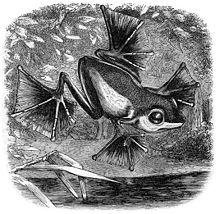
\includegraphics[width = .4\linewidth]{plus-1.jpeg} % 设定图片宽度相对于版心宽度,图片文件资源名
    \caption{华莱士在其著作《马来群岛》中绘制的飞蛙速写} % 图的题注
    \label{fig:plus-1} % 与 autoref 关联,设定交叉引用和显示「图x.x」
\end{figure}


% 梦里不觉 ☐ 已深, ☐ ☐ 岂是为他人。
\subparagraph{华莱士飞蛙} % +1s
华莱士飞蛙 (Rhacophorus nigropalmatus) ,
得名于它的发现者——生物学家阿尔弗雷德 · 华莱士 (Alfred R. Wallace)。
华莱士飞蛙生活在马来半岛的森林里,
它的体型很大,体长有 8 到 10 厘米,
除了交配和产卵,它们几乎从不下树……
如\autoref{fig:plus-1} 所示。

您是否注意到了,
源码中单个换行符并不会被编译成文档中的换行,
而两个或者超过两个换行符将开启一个新段落。
(类似HTML中新建了一个\texttt{<p>}标签)。
如果需要在文章中随意插入一个换行(类似于\texttt{<br>}标签),
则应该在源码文件中编写$\backslash\backslash$实现。
此标记一般仅在排版表格时使用,
或者活用于后期微调工作。

由于\LaTeX 的命令会使用几个固定的字符,
同其他编程语言处理字符串时一样,
当输出此类字符时需要使用逃逸策略,
如果您的论文编译错误,请\textbf{优先检查是否忘记逃逸此类字符}
\footnote{鄙人在写这份文档的时候都还是会忘记记给下划线逃逸(\LaTeX 命令使用下划线表示下标)}。
逃逸规则见\autoref{tab:escape} 所示。


% 和图一样,这里的htbp先不要管,先照抄
\begin{table}[htbp]
    \centering  % 依照规定 表格必须居中版心放置
    \caption{\LaTeX 命令专用字符逃逸规则} % 表格题注,zjuthesis.cls 将其设置在表格之上
    \label{tab:escape} % 交叉引用
    \begin{tabu}{lllllllll} % 9 列均左对齐
        \toprule % 头线
        输出 & \#  & \$  & \&  & \_  & \{   & \}  & \~{}  & \`{} \\ % 注意到了这个换行符吗
        \midrule % 中线
        源码 &  % 感受一下这里的「逃逸」
        \texttt{$\backslash$\#} &
        \texttt{$\backslash$\$} &
        \texttt{$\backslash$\&} &
        \texttt{$\backslash$\_} &
        \texttt{$\backslash$\{} &
        \texttt{$\backslash$\}} &
        \texttt{$\backslash$\~{}} &
        \texttt{$\backslash$\`{}}\\
        \bottomrule % 底线
    \end{tabu}
\end{table}

至于反斜杠本身的逃逸方法,请见上一段文字或表格的源码。

默认情况下,
多个空格符、水平制表符或单个换行符,
都仅会被编译成文档中的一个空格,
然而,和西文不同,中文的词与词之间是没有空格的,
所以本模板在XeCJK环境的初始化配置上取消了此类规则。
利用这样的改动,
您在编写论文时可按照您的行文思路随意换行,
不必担心产生多余的空格。
随着您的行文篇幅渐巨,
您将慢慢体会到这种编辑方式的优势——
\textbf{内容}与\textbf{样式}的分离。

输出英文半角双引号,需要在源码编写两个反引号(``grave'')。
而中文双引号则直接在源码中编写一对全角双引号即可。
鉴于目前大陆地区的官方标准明确规定使用此种方法标记引号,
请不要在论文中使用台湾地区和日本等地使用的直角引号
\footnote{网页中文排版近年来有惯用直角引号的趋势,此处不讨论}。

% 论文除了第一章绪论和终章的总结与展望, 最后都需要撰写一节“本章小结”。
% 活用注释作为 ToDo 提醒是一个好习惯
\section{本章小结}
本章简单描述了\LaTeX 排版的基本概念和本模板的源码结构,
通过同步实例介绍了最基本语义单元的编写。
现在,您可以尝试开始编写自己的论文,
当遇到无法排版的元素或无法解决的问题时,
欢迎继续阅读下一章。
